\documentclass{beamer}

\usepackage[utf8]{inputenc}
\usepackage[english]{babel}
\usepackage{textpos}
\usepackage{graphicx}
\usepackage{textcomp}
\usepackage{animate}
\usepackage{comment}
%\usepackage{multicol}
%\setlength{\columnsep}{5cm}
\usepackage{amsmath}
\usepackage{amsfonts}
\usepackage{verbatim}
\usepackage{varwidth}
\usepackage{caption}
\usepackage{dcolumn}
\usepackage{amssymb}
\usepackage{algorithm}
\usepackage{algorithmic}
%\usepackage{physics}
\usepackage{hyperref}
\usepackage{scalerel,stackengine}
\usepackage{fancyvrb}


\newcommand{\code}[1]{\texttt{#1}}
\newcommand{\shp}{$>>>$ }
\newcommand{\tab}{\hspace*{22pt}}

\usetheme{Madrid}

\title{Chapters 4 and 6: \\ Functions}
\author{EEC 3150}
\date{}

\institute{Trevecca Nazarene University}
 


%%%%%%%%% BEGIN DOCUMENT %%%%%%%%%
%%%%%%%%% BEGIN DOCUMENT %%%%%%%%%
%%%%%%%%% BEGIN DOCUMENT %%%%%%%%%

\begin{document}

% get title page 
\frame{\titlepage}
 
%%%%%%%%%%
%%%%%%%%%%
\begin{frame}	
	\frametitle{Outline}
	\tableofcontents	
\end{frame}


%%%%%%%%%%
%%%%%%%%%%
\section{Functions}

\begin{frame}	
	\center{\Huge{Functions}}
\end{frame}

\begin{frame}	
	\frametitle{Functions}
	
	\begin{block}{Motivating functions:}
		\begin{itemize}
			\item Consider the program we wrote that used bisection to approximate the square root of 2
			\item Suppose that we:\\
					1. wanted to find the root of a different number \\
					2. wanted a different order root \\
					3. wanted a different level of precision ($\epsilon$) \\
					4. were writing a program which needed to evaulate several roots
			\item All of these cases would require us to copy the code and change the variable values at each occurrence of the code (this is a pain)
			\item Instead, we can write a function that performs bisection by taking the parameters above (root order, argument of the root, precision) as input and returning the result and then simply call the function whenever we need it
		\end{itemize}
	\end{block}
	
\end{frame}

\begin{frame}%[fragile]
	\frametitle{Functions}
	
	\begin{alertblock}{Defn: function}
		\textbf{Functions} are essentially labeled blocks of code which can be called by using their label instead of manually copying the block of code (similar to how we can set \code{x = 10} and then use \code{x} instead of 10)
		
		\vspace{15pt}
		\minipage{0.5\textwidth}
			Prototypical function definition:
			
			\vspace{10pt}
			
			\code{def my\_function( \emph{arguments} ):\\
			\tab \emph{block of code} \\
			\tab return \emph{output}
			}
			
			\vspace{10pt}
			
			(Note: italics in code snippets mean "some code goes here")
		\endminipage\hfill
		\minipage{0.5\textwidth}
			\begin{itemize}
				\item Use the keyword \code{def} to start the function definition
				\item Name the function,
				\item List arguments (0 or more, comma-separated)
				\item End line with colon
				\item Indent the body of the function
				\item \code{return} any output 
			\end{itemize}
		\endminipage\hfill
	\end{alertblock}
	
\end{frame}

\begin{frame}%[fragile]
	\frametitle{Functions}
	
	\begin{block}{Example: hello function}
%		\vspace{15pt}
		\minipage{0.5\textwidth}
%			Prototypical function definition:
			
%			\vspace{10pt}
			
			\code{def hello( name ):\\
			\tab print(``hello, ``+name)
			}
			
%			\vspace{10pt}
			
%			(Note: italics in code snippets mean "some code goes here")
		\endminipage\hfill
		\minipage{0.5\textwidth}
			\begin{itemize}
				\item Accepts a string \code{name} as input
				\item Doesn't return anything, but prints to the console
			\end{itemize}
		\endminipage\hfill
		
		\vspace{15pt}
		
		Important points:
		\begin{itemize}
			\item Merely defining the function won't run anything
			\item It must be called (AFTER it's definition)
		\end{itemize}
	\end{block}
	
\end{frame}

\begin{frame}%[fragile]
	\frametitle{Functions}
	
	\begin{block}{Example: area of triangle}
%		\vspace{15pt}
		\minipage{0.6\textwidth}
%			Prototypical function definition:
			
%			\vspace{10pt}
			
			\code{def AreaOfTriangle( base, height ): \\
    			\tab return base*height/2 \\
			\# end
			}
			
%			\vspace{10pt}
			
%			(Note: italics in code snippets mean "some code goes here")
		\endminipage\hfill
		\minipage{0.4\textwidth}
			\begin{itemize}				
				\item Accepts \code{base,height} as arguments
				\item Returns \code{area}
			\end{itemize}
		\endminipage\hfill
	\end{block}
	
	\begin{block}{Example: sum $A$ to $B$}
%		\vspace{15pt}
		\minipage{0.5\textwidth}
%			Prototypical function definition:
			
%			\vspace{10pt}
			
			\code{def sumAtoB( A, B ): \\
    			\tab total = 0 \\
    			\tab for i in range(A,B+1): \\
        		\tab \tab total += i \\
    			\tab \# end \\
    			\tab return total \\
			\# end
			}
			
%			\vspace{10pt}
			
%			(Note: italics in code snippets mean "some code goes here")
		\endminipage\hfill
		\minipage{0.5\textwidth}
			\begin{itemize}
				\item Sums integers from A to B
				\item Accepts A and B as arguments
				\item \code{B+1} in \code{range()} since it stops one short
				\item Returns total
			\end{itemize}
		\endminipage\hfill
	\end{block}
	
\end{frame}

\begin{frame}%[fragile]
	\frametitle{Functions}
	
	\begin{block}{Example: defining several functions in one program}
		Calculate the diameter, perimeter, and area of a circle given the radius:
		
		\vspace{15pt}
		\minipage{0.6\textwidth}
			\code{def diameter( r ): \\
    			\tab return 2*r \\
			\# end
			}
			
			\vspace{10pt}
			
			\code{def perimeter( r ): \\
			\tab pi = 3.1415 \\
    			\tab return 2*pi*r \\
			\# end
			}
			
			\vspace{10pt}
			
			\code{def area( r ): \\
			\tab pi = 3.1415 \\
    			\tab return pi*r**2 \\
			\# end
			}
		\endminipage\hfill
		\minipage{0.4\textwidth}
			\begin{itemize}				
				\item We can define as many functions as we want
				\item Create a variable for \code{pi}
			\end{itemize}
		\endminipage\hfill
	\end{block}
	
\end{frame}


\begin{frame}%[fragile]
	\frametitle{Functions}
	
	\begin{block}{Example: calling a function from a function}
		Calculate the diameter and perimeter of a circle given the radius:
		
		\vspace{15pt}
		\minipage{0.6\textwidth}
			\code{def diameter( r ): \\
    			\tab return 2*r \\
			\# end
			}
			
			\vspace{10pt}
			
			\code{def perimeter( r ): \\
			\tab pi = 3.1415 \\
			\tab d = diameter( r ) \\
    			\tab return pi*d \\
			\# end
			}
		\endminipage\hfill
		\minipage{0.4\textwidth}
			\begin{itemize}				
				\item We can call \code{diameter} from \code{perimeter}
				\item We can even define \code{perimeter} before \code{diameter} (Python is smart enough to find \code{diameter} when interpreting the definition of \code{perimeter})
			\end{itemize}
		\endminipage\hfill
	\end{block}
	
\end{frame}

\begin{frame}%[fragile]
	\frametitle{Functions}
	
	\begin{block}{Example: bisection root}
		Let's now write our bisection root-finder as a function:
		
		\vspace{15pt}
		\minipage{0.5\textwidth}
			\begin{figure}[ht]
				\centering
				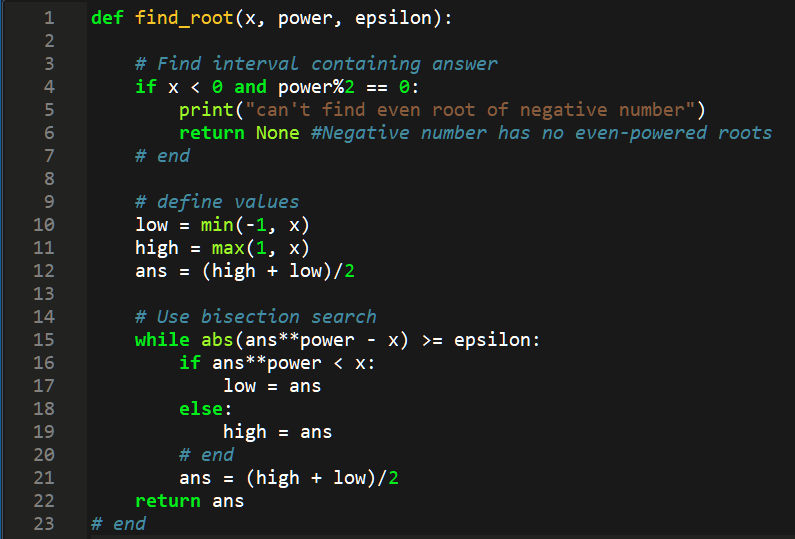
\includegraphics[width=0.9\linewidth]{RootFunction}
%				\caption{Visual depiction of the algorithm}
			\end{figure}
		\endminipage\hfill
		\minipage{0.5\textwidth}
			\begin{itemize}
				\item Accepts 3 arguments:\\
						1. \code{x}: the number to be ``rooted'' \\
						2. \code{power}: the power of the root \\
						3. \code{epsilon}: the error tolerance
				\item Returns \code{None} if it can't compute the root
			\end{itemize}
		\endminipage\hfill
	\end{block}
	
\end{frame}

\begin{frame}%[fragile]
	\frametitle{Functions}
	
	\begin{block}{Positional vs. keyword arguments:}
		There are 2 ways to provide arguments to Python:
		\begin{itemize}
			\item Positional: listing the arguments in order
				\item Keyword: listing them in any order but using their names
		\end{itemize}
		
		\vspace{10pt}		
		\code{def print\_name(first, last): \\
				\tab print(first, last) \\
				\# end \\
				\tab \\
				print\_name( 'walter', 'white' ) \\
				print\_name( first='walter', last='white' ) \\
				print\_name( last='white', first='walter' )
		}
		\vspace{10pt}		
		
		NOTE: any positional arguments must come BEFORE ALL keyword arguments
	\end{block}
	
\end{frame}

\begin{frame}%[fragile]
	\frametitle{Functions}
	
	\begin{block}{Default values for arguments:}
		You can set the default value of an argument in the first line of a function definition (this value will be used if you don't supply the argument when calling the function):
		
		\vspace{10pt}	
		\code{def print\_name(first, last='white'): \\
				\tab print(first, last) \\
				\# end \\
				\tab \\
				print\_name( 'walter' ) \\
				print\_name( 'walter', 'white' ) \\
				print\_name( first='walter', last='white' ) \\
				print\_name( last='white', first='walter' )
		}
		\vspace{10pt}		
		
		NOTE: any keyword arguments must come AFTER ALL positional arguments
	\end{block}
	
\end{frame}


\begin{frame}%[fragile]
	\frametitle{Functions}
	
	\begin{block}{Variable number of arguments:}
		Like with \code{max()} function, you can provide a variable number of arguments to a Python function by using the \emph{unpacking operator} (*):
		
		\vspace{10pt}
		\minipage{0.5\textwidth}
			\code{def mean( *args ):\\
					\tab tot = 0 \\
					\tab for a in args: \\
					\tab \tab tot += a \\
					\tab \# end \\
					\tab return tot/len(args) \\
					\# end
			}
			
%			\vspace{10pt}
			
%			(Note: italics in code snippets mean "some code goes here")
		\endminipage\hfill
		\minipage{0.5\textwidth}
			\begin{itemize}
			\item \code{args} is a \emph{tuple} (a sequence of values, more on that in the next chapter)
			\item \code{len()} is a function which returns how many elements are in a tuple (also works for strings)
			\item Like with strings, you can index individual elements using brackets []: \code{args[0]} will give the 0th element
			\end{itemize}
		\endminipage\hfill
	\end{block}
	
\end{frame}

\begin{frame}%[fragile]
	\frametitle{Functions}
	
	\begin{exampleblock}{Exercise: \code{max()}:}
		Let's write our own version of the \code{max()} function (HINT: float(`-inf') will be useful)
	\end{exampleblock}
	
\end{frame}

\begin{frame}%[fragile]
	\frametitle{Functions}
	
	\begin{block}{Multiple returns:}
		Functions can also return multiple values:
		
		\vspace{10pt}
		\minipage{0.5\textwidth}
			\code{def DiamPerim( r ): \\
			\tab d = 2*r \\
			\tab pi = 3.1415 \\
			\tab p = pi*d \\
    			\tab return d, p \\
			\# end \\
			\tab \\
			d, p = DiamPerim( 10 )
			}
			
%			\vspace{10pt}
			
%			(Note: italics in code snippets mean "some code goes here")
		\endminipage\hfill
		\minipage{0.5\textwidth}
			\begin{itemize}
			\item Separate returned values with commas
			\end{itemize}
		\endminipage\hfill
	\end{block}
	
\end{frame}


%%%%%%%%%%
%%%%%%%%%%
\section{Scoping}

\begin{frame}	
	\center{\Huge{Scoping}}
\end{frame}

\begin{frame}%[fragile]
	\frametitle{Scoping}
	
	\begin{block}{Example: scoping}
%		\vspace{15pt}
		\minipage{0.5\textwidth}
			What will this code do?
			
			\vspace{10pt}
			
			\code{def f():\\
			\tab x = 1 \\
			\#  end \\
			\tab \\
			print(x)
			}
		\endminipage\hfill
		\minipage{0.5\textwidth}
			
		\endminipage\hfill
	\end{block}
	
\end{frame}

\begin{frame}%[fragile]
	\frametitle{Scoping}
	
	\begin{block}{Example: scoping}
%		\vspace{15pt}
		\minipage{0.35\textwidth}
			What will this code do?
			
			\vspace{10pt}
			
			\code{def f():\\[-3pt]
			\tab x = 1 \\[-3pt]
			\#  end \\[6pt]
			print(x)
			}
		\endminipage\hfill
		\minipage{0.65\textwidth}
			\begin{itemize}
				\item This code will not run
				\item Since \code{x} was defined in \code{f}, it can only be accessed inside \code{f}
				\item Even calling \code{f()} won't make it work
				\item The \emph{scope} of \code{x} is only the function \code{f}
			\end{itemize}
		\endminipage\hfill
	\end{block}
	
	\begin{alertblock}{Defn: scoping}
		The \textbf{scope} of an object in Python (or any programming language) the section(s) of a program in which the object is defined and can be accessed
		
		\vspace{10pt}
		Consequences:
			\begin{itemize}
				\item Variables/functions may not be acllable in some parts of the code
				\item The same variable name may refer to different objects in different section of code
			\end{itemize}
	\end{alertblock}
	
\end{frame}

\begin{frame}%[fragile]
	\frametitle{Scoping}
	
	\begin{block}{Example: scoping}
%		\vspace{15pt}
		\minipage{0.5\textwidth}
			What will this code do?
			
			\vspace{10pt}
			
			\code{def f(x):\\[-3pt]
			\tab print(x) \\[-3pt]
			\#  end \\[6pt]
			f(1) \\
			print(x)
			}
		\endminipage\hfill
		\minipage{0.5\textwidth}
			\begin{itemize}
				\item Scoping also applies to the arguments of functions
				\item \code{x} can't be accessed outside the function
				\item Of course, we could define a new \code{x} variable outside the function, but it would have no relation to the one inside the function
			\end{itemize}
		\endminipage\hfill
	\end{block}
	
\end{frame}

\begin{frame}%[fragile]
	\frametitle{Scoping}
	
	\begin{block}{Example: scoping}
		\minipage{0.5\textwidth}
			\code{def f():\\
			\tab print(x) \\
			\tab \# x += 1 \\
			\#  end \\
			\tab \\
			x = 1 \\
			f()
			}
		\endminipage\hfill
		\minipage{0.5\textwidth}
			\begin{itemize}
				\item There are \code{x} variables both inside \code{f()} and the program (module) it's defined within
				\item Running the program as it is will print 1 (without a separate definition of \code{x} specifically for \code{f}, it assumes that the module's value of \code{x} is what we want)
				\item However, if we uncomment \code{x = 2}, then \code{f} now has its own definition of \code{x}, which it tried to access (by printing) before it was defined
			\end{itemize}
		\endminipage\hfill
	\end{block}
	
\end{frame}

\begin{frame}%[fragile]
	\frametitle{Scoping}
	
	\begin{alertblock}{Defn: global vs. local variables}
		\begin{itemize}
			\item \textbf{Local variables}: variables with a limited scope (usually limited to a certain function or class)
			\item \textbf{Global variables}: variables with an unlimited scope that can be accessed from ANY function via the \code{global} keyword
		\end{itemize}
		
		\vspace{10pt}
		\minipage{0.5\textwidth}
			\code{def f():\\
			\tab global x \\
			\tab x += 1 \\
			\#  end \\
			\tab \\
			x = 1 \\
			f() \\
			print(x)
			}
		\endminipage\hfill
		\minipage{0.5\textwidth}
			\begin{itemize}
				\item The \code{x} defined outside of \code{f} is global, but \code{f} can't modify it
				\item Normally, any \code{x} defined within \code{f} would be local (its scope would be limited to \code{f}
				\item However, using the \code{global} keyword inside \code{f} allows the function to change \code{x}
			\end{itemize}
		\endminipage\hfill
	\end{alertblock}
	
\end{frame}

\begin{frame}%[fragile]
	\frametitle{Scoping}
	
	\begin{block}{Example: nested scoping}
%		\vspace{15pt}
		\minipage{0.35\textwidth}
			Let's explore this code:
			
			\vspace{10pt}
			
			\code{def f():\\
			\tab def g() \\
			\tab \tab y = 2 \\
			\tab \#  end \\[6pt]
			\tab x = 1 \\
			\# end
			}
		\endminipage\hfill
		\minipage{0.65\textwidth}
			What it does:
			\begin{itemize}
				\item Defines a function \code{f}
				\item Objects whose scope is \code{f}: \code{x, g()}
				\item Objects whose scope is \code{g}: \code{x, y}
			\end{itemize}
			Let's try:
			\begin{itemize}
				\item Calling \code{f()}
				\item Calling \code{g()} in \code{f()}
				\item Printing values of variables to test scoping
				\item Define \code{z} outside both functions
			\end{itemize}
		\endminipage\hfill
	\end{block}
	
\end{frame}

\begin{frame}%[fragile]
	\frametitle{Scoping}
	
	\begin{alertblock}{Defn: call stack and frame}
		\minipage{0.4\textwidth}
			\begin{itemize}
				\item A \textbf{call stack} is a data structure which stores information about currently active functions within a program
				\item A \textbf{frame} is an item in the call stack which refers to a particular function
				\item We say that frames are \emph{pushed onto} and \emph{popped off of} the stack
			\end{itemize}
		\endminipage\hfill
		\minipage{0.6\textwidth}
			\begin{figure}[ht]
				\centering
				
\includegraphics[width=0.9\linewidth]{CallStack}
				\caption{Source: towardsdatascience.com}
			\end{figure}
		\endminipage\hfill
	\end{alertblock}
	
\end{frame}

\begin{frame}%[fragile]
	\frametitle{Scoping}
	
	\begin{block}{Call stack and errors:}
		One place where understanding how a call stack works in when debugging errors:
		
		\vspace{15pt}
		
		\minipage{0.5\textwidth}
			\code{def f():\\
			\tab return 1+'c' \\
			\# end \\
			f()
			}
		\endminipage\hfill
		\minipage{0.5\textwidth}
			\begin{itemize}
				\item This code will throw an error because we can't add an integer and a string
				\item The error message will acknowledge that the error occurred in \code{f()}
			\end{itemize}
		\endminipage\hfill
	\end{block}
	
\end{frame}

\begin{frame}%[fragile]
	\frametitle{Scoping}
	
	\begin{block}{Call stack and errors}
		One place where understanding how a call stack works in when debugging errors:
		
		\vspace{15pt}
		\minipage{0.5\textwidth}
			\code{def f():\\
			\tab def g() \\
			\tab \tab return 1+'c' \\
			\tab \#  end \\
			\tab g() \\
			\# end \\
			f()
			}
		\endminipage\hfill
		\minipage{0.5\textwidth}
			\begin{itemize}
				\item This code will throw an error because we can't add an integer and a string
				\item The error message will acknowledge that the error occurred in \code{g()} INSIDE \code{f()}
			\end{itemize}
		\endminipage\hfill
	\end{block}
	
\end{frame}


%%%%%%%%%%
%%%%%%%%%%
\section{Functions as Objects and Higher-Order Programming}

\begin{frame}	
	\center{\Huge{Functions as Objects \\ and \\[10pt] Higher-Order Programming}}
\end{frame}

\begin{frame}%[fragile]
	\frametitle{Functions as Objects and Higher-Order Programming}
	
	\begin{block}{Functions as Objects:}
		\minipage{0.5\textwidth}
			\code{def abs2(x, F, G): \\
					\tab if x > 0: \\
					\tab \tab return F(x) \\
					\tab else: \\
					\tab \tab return G(x) \\
					def f(x): \\
					\tab return x \\
					def g(x): \\
					\tab return -x \\
			}
		\endminipage\hfill
		\minipage{0.5\textwidth}
			\begin{itemize}
				\item Functions are objects just like \code{int}'s and \code{float}'s
				\item Try \code{type(abs)}
				\item Therefore, you can pass/return functions to/from other functions
				\item This is called \emph{higher-order programming}
			\end{itemize}
		\endminipage\hfill
	\end{block}
	
\end{frame}


%%%%%%%%%%
%%%%%%%%%%
\section{Recursion}

\begin{frame}	
	\center{\Huge{Recursion}}
\end{frame}

\begin{frame}%[fragile]
	\frametitle{Recursion}
	
	\begin{block}{Defn: factorial}
		The factorial function takes an integer and multiplies all positive integers up to (and including) itself:
		\begin{equation*}
			n! = n(n-1)(n-2) \cdots 3 \cdot 2 \cdot 1
		\end{equation*}
%		\vspace{10pt}
		It can be more properly defined in an inductive/recursive fashion using the following recurrence relation:
		\begin{equation*}
			\begin{split}
				1! & = 1 \\
				n! & = n\cdot(n-1)!
			\end{split}
		\end{equation*}	
%		\vspace{10pt}
		This second definition gives us a different perspective on how it operates (and, thus, how to code it)
	\end{block}
	
\end{frame}

\begin{frame}%[fragile]
	\frametitle{Recursion}
	
	\begin{block}{Two ways to write a factorial function:}
		\minipage{0.5\textwidth}
			\code{def fact1(n): \\
					\tab ans = 1 \\
					\tab for i in range(1,n+1): \\
					\tab \tab ans *= i \\
					\tab return ans
			}
		\endminipage\hfill
		\minipage{0.5\textwidth}
			\code{def fact2(n): \\
					\tab if n == 1: \\
					\tab \tab return 1 \\
					\tab else: \\
					\tab \tab return n*fact2(n-1)
			}
		\endminipage\hfill
		
		\vspace{10pt}
		\begin{itemize}
			\item The first function simply uses a for loop to loop through all the relevant integers (in the style of the first definition of factorial)
			\item The second function actually calls itself with an argument one less than the previous call to compute factorial (in the style of the second definition)
			\item The second function is an example of \emph{recursion}
		\end{itemize}
	\end{block}
	
\end{frame}

\begin{frame}%[fragile]
	\frametitle{Recursion}
	
	\begin{alertblock}{Defn: recursion}
		In general, \textbf{recursion} is a technique for solving a problem which breaking into simpler version of the same problem
		\begin{itemize}
			\item In a programming context, this consists of making a function call itself in such a way that after each recursive call, the problem gets simpler
			\item Ex: each time \code{fact2()} calls itself, the argument is one less
		\end{itemize}
		Parts of a recursive function (you can have one or more of each):
		\begin{itemize}
			\item Recursion case: where the function calls a simpler version of itself
			\item Base case: the simplest possible case where recursion finally ends
		\end{itemize}
		Without a base case, there will be ``infinite'' recursion (rather recursion until the call stack gets full and you run out of memory)
	\end{alertblock}
	
\end{frame}

\begin{frame}%[fragile]
	\frametitle{Recursion}
	
	\begin{block}{Recursive factorial cases:}
		\minipage{0.5\textwidth}
			\code{def fact2(n): \\
					\tab if n == 1: \\
					\tab \tab return 1 \\
					\tab else: \\
					\tab \tab return n*fact2(n-1)
			}
		\endminipage\hfill
		\minipage{0.5\textwidth}
			\begin{itemize}
				\item Base case: \\
					\code{return 1}
				\item Recursion case: \\
					\code{return n*fact2(n-1)}
			\end{itemize}
		\endminipage\hfill
	\end{block}
	
\end{frame}

\begin{frame}%[fragile]
	\frametitle{Recursion}
	
	\begin{exampleblock}{Fibonacci sequence:}
		The Fibonacci sequence $F(n)$ is defined recursively as follows:
		\begin{equation*}
			\begin{split}
				F(0) & = 0 \\
				F(1) & = 1 \\
				F(n) & = F(n-1)+F(n-2)
			\end{split}
		\end{equation*}
		Write a recursive and a non-recursive Fibonacci function
	\end{exampleblock}
	
\end{frame}


%%%%%%%%%%
%%%%%%%%%%
\section{Using Functions to Modularize Code}

\begin{frame}	
	\center{\Huge{Using Functions to Modularize Code}}
\end{frame}

\begin{frame}%[fragile]
	\frametitle{Modularizing with Functions}
	
	\begin{alertblock}{Defn: modularization}
		\textbf{Modularization} is the process of writing large programs using many smaller sub-programs (aka, functions), thus making the code more organized and readable
	\end{alertblock}
	
	\begin{exampleblock}{Modularizing the hyperbolic trig functions:}
		\minipage{0.5\textwidth}
			Here are the hyperbolic \\ trig functions:
			\begin{equation*}
				\begin{split}
					sinh(x) & = \frac{e^x-e^{-x}}{2} \\
					cosh(x) & = \frac{e^x+e^{-x}}{2} \\
					tanh(x) & = \frac{sinh(x)}{cosh(x)} = \frac{e^x-e^{-x}}{e^x+e^{-x}} \\
				\end{split}
			\end{equation*}
		\endminipage\hfill
		\minipage{0.5\textwidth}
			Write several Python functions:
			\begin{itemize}
				\item an exponential function
				\item a function for each trig function
				\item a function which returns all trig functions
			\end{itemize}
			NOTE: each function will use the one before it
		\endminipage\hfill
		
	\end{exampleblock}
	
\end{frame}


%%%%%%%%%%
%%%%%%%%%%
\section{Specifications}

\begin{frame}	
	\center{\Huge{Specifications}}
\end{frame}

\begin{frame}%[fragile]
	\frametitle{Specifications}
	
	\begin{block}{help():}
		Run these commands in the console:
		
		\vspace{15pt}
		\minipage{0.5\textwidth}
			\code{help(abs) \\
			help(max) \\
			help(len) \\
			help(print) \\
			}
		\endminipage\hfill
		\minipage{0.5\textwidth}
			\begin{itemize}
				\item The \code{help()} function provides info about functions (and other objects)
				\item Prints the name, arguments, and description of a function
				\item The descriptions come from something called a \emph{docstring} (let's make our own example)
			\end{itemize}
		\endminipage\hfill
	\end{block}
	
\end{frame}

\begin{frame}%[fragile]
	\frametitle{Specifications}
	
	\begin{block}{Docstring:}
		Define this function and run \code{help()} on it:
		
		\vspace{15pt}
		\minipage{0.5\textwidth}
			\code{def f(x): \\
			\tab ''' \\
			\tab this is a docstring \\
			\tab ''' \\
			\tab return x+1 \\
			\# end \\
			\tab \\
			help(f)
			}
		\endminipage\hfill
		\minipage{0.5\textwidth}
			\begin{itemize}
				\item Triple quotes define a multi-line comment (single or double)
				\item When placed at the beginning of a function definition, they make something called a \textbf{docstring}
				\item Docstrings are used to describe the purpose of the function (see the previous examples)
				\item i.e., docstrings provide the \textbf{specifications} of a function
			\end{itemize}
		\endminipage\hfill
	\end{block}
	
\end{frame}

\begin{frame}%[fragile]
	\frametitle{Specifications}
	
	\begin{block}{Example: docstring}
		\minipage{0.5\textwidth}
			\code{def mean( *args ):\\
					\tab ''' \\
					\tab This function returns \\
					\tab the mean of the \\
					\tab variable number of \\
					\tab arguments (float or int) \\
					\tab provided \\
					\tab ''' \\
					\tab tot = 0 \\
					\tab for a in args: \\
					\tab \tab tot += a \\
					\tab \# end \\
					\tab return tot/len(args) \\
					\# end
			}
		\endminipage\hfill
		\minipage{0.5\textwidth}
			\begin{itemize}
			\item Here is our \code{mean} code with a docstring providing its specification
			\end{itemize}
		\endminipage\hfill
	\end{block}
	
\end{frame}






\end{document}




